%%%%%%%%%%%%%%%%%%%%%%% file template.tex %%%%%%%%%%%%%%%%%%%%%%%%%
%
% This is a general template file for the LaTeX package SVJour3
% for Springer journals.          Springer Heidelberg 2010/09/16
%
% Copy it to a new file with a new name and use it as the basis
% for your article. Delete % signs as needed.
%
% This template includes a few options for different layouts and
% content for various journals. Please consult a previous issue of
% your journal as needed.
%
%%%%%%%%%%%%%%%%%%%%%%%%%%%%%%%%%%%%%%%%%%%%%%%%%%%%%%%%%%%%%%%%%%%
%
% First comes an example EPS file -- just ignore it and
% proceed on the \documentclass line
% your LaTeX will extract the file if required
\begin{filecontents*}{example.eps}
%!PS-Adobe-3.0 EPSF-3.0
%%BoundingBox: 19 19 221 221
%%CreationDate: Mon Sep 29 1997
%%Creator: programmed by hand (JK)
%%EndComments
gsave
newpath
  20 20 moveto
  20 220 lineto
  220 220 lineto
  220 20 lineto
closepath
2 setlinewidth
gsave
  .4 setgray fill
grestore
stroke
grestore
\end{filecontents*}
%
\RequirePackage{fix-cm}
%
%\documentclass{svjour3}                     % onecolumn (standard format)
%\documentclass[smallcondensed]{svjour3}     % onecolumn (ditto)
\documentclass[smallextended]{svjour3}       % onecolumn (second format)
%\documentclass[twocolumn]{svjour3}          % twocolumn
%
\usepackage{kotex}                           % https://crmn.tistory.com/34

\smartqed  % flush right qed marks, e.g. at end of proof
%
\usepackage{graphicx}
%
% \usepackage{mathptmx}      % use Times fonts if available on your TeX system
%
% insert here the call for the packages your document requires
%\usepackage{latexsym}
% etc.
%
% please place your own definitions here and don't use \def but
% \newcommand{}{}
%
% Insert the name of "your journal" with
% \journalname{myjournal}
%

\begin{document}

\bibliographystyle{spbasic} % Choose Phys. Rev. style for bibliography
 
\title{비잔틴 장애를 허용하는 실용적인 상태 복제 알고리즘에 대한 조사 및 분석%\thanks{Grants or other notes
%about the article that should go on the front page should be
%placed here. General acknowledgments should be placed at the end of the article.}
}
% \subtitle{Do you have a subtitle?\\ If so, write it here}

%\titlerunning{Short form of title}        % if too long for running head

\author{최창원         \and
        조은선 %etc.
}

%\authorrunning{Short form of author list} % if too long for running head

\institute{최창원 \at
              충남대학교
              \email{qwefgh90@naver.com}           %  \\
%             \emph{Present address:} of F. Author  %  if needed
           \and
              조은선 \at
              충남대학교
              \email{eschough@cnu.ac.kr}
}

\date{작성일: 2020/12/08}
% The correct dates will be entered by the editor


\maketitle

\renewcommand{\abstractname}{초록}
\begin{abstract}
본 서베이 논문은 비잔틴 장애를 허용(Byzantine-fault-tolerant)하는 
상태 머신 복제(State Machine Replication) 알고리즘과 블록체인의 분산 원장에 활용되는 기술 등을 다룬다. 
많은 수의 기업들은 정보 시스템을 활용하는 사업 아이템을 구상하고 있으며
IT 시스템에 대한 의존성은 높아지고 있다.
그리고 개발 비용을 절감하면서 생산성을 높이고 더 안정적인 시스템을 구축하기위해
타사의 API 서비스나 클라우드를 이용하여 새로운 시스템을 개발하는 추세이다.
그래서 현대의 대부분의 서비스는 분산된 노드가 서로 정보를 주고 받으며 동작한다.
이 과정에서 분산된 노드간에 동일한 설정 유지할때나 하나의 상태를 갖는 분산 컴포넌트를 개발할때
상태 머신 복제 알고리즘은 중요한 역할을 하게 된다.
상태 복제 알고리즘은 오랫동안 연구되어 왔으며 최근 블록체인의
발전으로 그 중요성이 부각되고 있다. 또한 HotStuff 같은 알고리즘의 등장으로 성능이 획기적으로
개선되기도 하였다. 이 서베이 논문은 비잔틴 장애 허용 알고리즘을 다루고
알고리즘 간에 성능 및 장단점을 비교하여 설명한다.

% \keywords{First keyword \and Second keyword \and More}
% \PACS{PACS code1 \and PACS code2 \and more}
% \subclass{MSC code1 \and MSC code2 \and more}
\end{abstract}

\section{서론}
\label{intro}
소프트웨어의 이미 제작된 컴포넌트를 재활용할 수 있는 장점 덕분에 
아이디어만 있다면 새로운 앱을 구현하는데 많은 시간을 들이지 않을 수 있다.
언어와 개발 도구의 발달, 오픈소스와 생태계의 발전, 웹 기술의 발전은 
재활용 가능한 소프트웨어를 누구나 쉽게 구현하고 제공할 수 있게 하였다.
단순한 라이브러리나 프레임워크 수준을 넘어선 API 서비스의 등장으로
코드 뿐만 아니라 서비스 자체를 재활용하는 것이 가능해졌다. 분산된 노드의
통신이 빈번한 환경에서는 악의적인 공격자에 의해 해킹을 당하기 쉽다.
해커는 시스템 중 약한 부위를 공격하여 루트권한을 획득하고 제어서버를 통해 
시스템을 원하는 대로 조작할 수 있다. 위와 같은 분산된 환경에서 해커의 공격을
대응하는 것이란 개발자 입장에서 단순히 시스템의 장애를 해결하는 것
이상의 어려운 일이다. 또한 점점 시스템에 많고 중요한 데이터가 저장되기 때문에 악의적인 공격을
당했을때 그 피해는 어마어마하다. 

다양한 분산 환경 중 여러 노드가 하나의 시스템 처럼
동일한 상태를 유지하고 서비스를 제공하는 경우가 있다.
특히 악의적인 노드가 존재하는 비잔틴 문제가 있더라도 시스템이
중요한 동작할 수 있게 해주는 비잔틴 장애 허용 상태 머신 복제 알고리즘은
보안성을 강화하기 위해 널리 활용되는 알고리즘이 되었다.
항상 시스템을 보호해주는 알고리즘은 아니고 \(3f+1\)개의 노드 중 f개 이하로 
결함있는 노드가 유지될때 문제없이 상태를 복제할 수 있게한다.

흔히 알려진 것 처럼 상태 머신 복제 시스템은 safety와 liveness 성질을 가
지고 있어야 한다. safety는 사용자가 전송한 시스템의 상태를 갱신하는 일련의
명령을 모든 노드가 동일한 순서대로 실행하여 같은 상태를 갖게해주는 능력이다.
liveness는 사용자 요청에 대한 응답을 해주는 능력을 의미한다.

동기적인(Synchronous) 모델은 유한한 제한 시간이 있어서 공격자가 결함없는 노드의 메시지를
그 시간 만큼만 지연시킬 수 있는 모델을 의미한다.
비동기적인(Asynchronous) 모델은 공격자가 제한할 수 있는 시간에는 제한이 없지만 
결함없는 노드가 보낸 메시지는 메시지는 결국 도달해야 되는 모델을 의미한다.
부분 동기화(Partial synchrony) 모델은 일시적인 순간에만 비동기적 모델을 유지하고(공격 받는 상황) 나머지 시간에는 동기적
속성을 유지하는 모델이다. 이 모델에는 전송 제한 시간과 GST(Global Stabilization Time)이 있다고 가정한다.

\begin{itemize}
  \item GST는 알려지지 않은 유한한 시간이 지난 시점이다.
  \item t라는 시점에 전송된 모든 메시지는 \(max\{t,GST\}+\Delta\) 안에 도달한다.
\end{itemize}


최근에 상태 복제 머신이 활용되는 분야 중 하나는 블록체인(Blockchain)이
다. 블록체인은 동일한 기록을 갖는 분산원장으로 구성된다. 일반적으로 모든
분산 원장은 동일한 암호화페 거래내역을 저장해야 하며, 거래 요청 처리 순서를
동기화하여 처리해야 한다. 여기서 각 분산된 노드의 상태는 계좌내역(계좌번호,
잔액 등)이고, 이 상태를 모두 동일하게 복제하기 위해 상태 머신 복제 알고리즘이
사용된다.

예를들어 비트코인은 작업증명(Proof of Work) 알고리즘과 Longest Chain
Rule을 활용하여 상태를 복제한다. 여러 복제본이 Proof of Work를 통해 블록 블록을
찾은 뒤 전파하여 동기화하고 Longest Chain Rule을 이용하여 포크 문제를 해결한다.
작업증명 알고리즘은 본래 서비스 거부 공격을 방어하기 위해 개발되었지만, 
비트코인에서 각 노드간 동일한 블록체인을 동기화할때 사용되면서 유명해졌다.

초기 버전 이더리움 같은 경우도 ethash를 적용한 작업증명 알고리즘과 고스트 프로토콜을
이용하여 상태 복제를 수행하고 및 포크 문제를 다루었다. 블록체인은 이처럼 초기에는 
서비스 거부 공격을 방어할 수 있는 작업증명 같은 보안성이 강한 알고리즘을 채택하였다.
이러한 시스템을 붕괴하기 위해서는 비잔틴 노드가 전체 노드의 51\% 이상이 되어야 하므로
해커들 입장에서도 해킹에 필요한 비용이 너무 비싸서 블록체인 자체를 공격하는 것은
어렵다고 한다.

하지만 블록체인 특성상 지리적으로 떨어진 노드가 많아서 포크 문제가 빈번하게 발생했고
Ghost 프로토콜 등을 이용해 이 문제를 다룰 수 있더라도, 한쪽 블록 전체를 버리게 됨으로써 
블록을 낭비하는 문제는 여전히 남아있었다. 그래서 이더리움 2.0에서는 지분증명과
같은 알고리즘을 지원하기 시작하였다.

블록체인 분야에서 사용되기도 하는
가장 널리 알려진 PBFT(Practical Byzantine Fault Tolerance)는 비동기 환경에서 비잔틴 문제를 해결할 수 있는
최초의 알고리즘이다. 순서 합의부터 결과 커밋까지 3가지 단계 Pre-Prepare, Prepare,
Commit로 구성되며 Pre-Prepare과 Prepare 단계는 동일한 순서로 명령이 실
행되는 것을 보장하며, Prepare과 Commit 단계는 커밋된 명령이 여러 뷰에서
완전히 정렬되는 것을 보장한다. 이후 PBFT의 성능을 개선한 많은 변형이 탄생
하였다. 현대에 쓰기에는 다소 성능이 느린 문제가 있다.

그리고 2019년 현대 시스템 환경에서 PBFT보다 빠르고 실용적인 리더 기반
상태 머신 복제 알고리즘 HotStuff가 등장하였다. HotStuff는 리더 기반 프로토
콜로 부분적으로 동기 모델(Partially Synchronous Model)에서 동작하는 상태
머신 복제 알고리즘이다. 네트워크 커뮤니케이션이 동기적일때 네트워크 지연시
간의 속도에 맞춰 합의에 도달할 수 있게 해주는 responsiveness 속성을 보장한다.
그리고 복제본의 수에 선형적인 통신 복잡도를 갖는 linearity를 보장한다. 아마
HotStuff는 위 2가지 속성을 갖는 최초의 부분 동기화 BFT 복제 프로토콜이며,
거대한 복제 서비스에서 활용될 수 있는 여러가지 성능 최적화를 제공한다.

그리고 같은 해인 2019년에 LibraBFT라는 Libra 블록체인을 위한 알고리
즘이 등장한다. LibraBFT는 HotStuff 알고리즘을 기반으로 몇가지 아이디어가
추가된 알고리즘이다. LibraBFT는 새로운 라운드 동기화 매커니즘을 제공하며,
결함있는 리더 노드가 존재하더라도 제안이 커밋되는 것을 허용하는 nil-block
투표 방식 등을 제공한다.


\section{논문 분석}
\label{sec:1}
주로 블록체인(Blockchain)에서 활용되는 합의(Consensus) 알고리즘이나
널리 알려진 상태 머신 복제(State Machine Repliacation)을 요약하고
각 알고리즘의 특징과 장단점 등을 설명할 것이다. 그리고 시스템 설계나
블록체인을 연구하는 관점에서 각 알고리즘을 분석한 내용을 포함할 것이고
실제 오픈소스나 실 운영되는 서비스에는 어떤 것이 있고 
미래에 활용될 수 있는 분야를 제시하고 시나리오도 함께 제시할 것이다.

\subsection{Practical Byzantine Fault Tolerance}
정부나 산업에서 점점 정보시스템에 대한
의존성이 커지면서 악의적인 공격이 성공하였을때 그 피해가 점점 커지게 되었다.
그리고 시스템에 점점 많은 기능이 들어가고 복잡해지면서 소프트웨어 버그가 많아지게 되었다.
그래서 자의적인 행동을 하는 비잔틴 행동(Byzantine behavior)으로 부터 시스템을
보호하는 비잔틴 장애 허용 알고리즘의 중요성이 커지게 되었다.

PBFT(Pratical Byzantine Fault Tolerance)는
1999년 Miguel Castro와 Barbara Liskov가 작성한 상태 머신 복제 알고리즘이다.
당시 이 논문이 발표되기전 소개되었던 알고리즘들은 동기적 환경에서 동작하거나
실제로 사용되기에는 너무 느렸다. 그래서 인터넷 환경과 같은 비동기 환경에서
비잔틴 문제를 허용하는 알고리즘이 필요하였고 PBFT가 등장하였다. 이 알고리즘은
결함있는 노드가 많아도 \([\frac{n-1}{3}]\)개 일때 safety와 liveness를 제공한다.

PBFT 이전에 등장한 알고리즘은 문제점을 크게 2가지 문제를 가지고 있었다. 
먼저 이론적으로 가능한지만 구현해서 사용하기에는 비효율적이고 어려웠다는 것이고
메시지 지연 시간과 처리 속도의 상한 값을 고정하는 동기화 가정(Synchrony Assumption)을 적용했다는 것이다.
Rampart나 SecureRing같은 알고리즘은 실용적이지만 정확성을 위해 동기화 가정에 의존하고 있었다.
동기화 가정은 악의적인 가정에 매우 취약하다. 공격자는 결함없는 노드를 그들 사이의 통신을 지연시키고
그 노드들이 결함있게 여겨지거나 복제 그룹에 의해 배제 당하게끔 하여 서비스의 안정성에 손상을 일으킬 수 있다.
PBFT는 동기화 가정에 의존하지 않기 때문에 저런 공격에 내성을 지니고 있다.

이 알고리즘은 상태 머신 복제 알고리즘이며 분산된 노드의 구성은 뷰(View)라는 단위로 관리된다.
뷰는 Primary와 여러개의 Backup으로 구성된다.
Primary는 사용자의 요청을 처리하기 위해 프로토콜을 시작하는 역할을 하는 복제본이다.
그리고 알고리즘의 동작을 위해 2가지 요구사항이 필요하다.
모든 복제본은 같은 순서의 요청 실행에 같은 상태를 갖도록 하기 위해
\textit{결정적(Deterministic)} 속성을 가져야하며 초기에 동일한 상태에서 시작해야 한다.

그리고 safety와 liveness 속성을 유지하기 위해 반드시 충족해야할 \(3f+1\)이라는 조건도 존재한다.
\(3f+1\)은 safety와 liveness를 위한 최소한의 복제본 숫자이다. 여기서 f는 결함있는 노드를 의미한다.
\(n\)개의 복제본이 있을때 f개의 응답하지 않는 결함있는 노드가 있을 수 있으며, f개의 결함이 있으나 응답하는 노드
f개의 결함이 있으나 응답하지 않는 노드가 있을 수 있다. 이때 메시지를 보내는 정상적인 노드의 개수는 결함을 가진
응답하는 노드의 개수보다 많아야 한다. 이는 수식으로 \(n-2f > f\) 즉, \(n >= 3f+1\)로 표현되고
이 조건이 만족되었을때 위의 2가지 속성이 보장되는 것이다.

이러한 필수적인 가정 외에 가정은 생략한다. primary가 사용자 요청 \textit{m} 받으면서 3단계 프로토콜을 시작한다.
3단계는 pre-prepare, prepare, commit이며 pre-prepare과 prepare 단계는
같은 뷰에 있는 여러개의 요청 순서를 정렬하기 위해 존재한다.
prepare, commit 단계는 모든 뷰를 거쳐 커밋된 요청들의 순서를 정렬하기 위해 존재한다.

먼저 pre-prepare 단계에서는 primary는 요청에 시퀀스 번호 \(n\)을 요청에 할당한다.
그리고 pre-prepare 메시지 \(((PRE-PREPARE,v,n,d)_{\sigma_{p}}),m)\)
를 모든 복제본에 멀티캐스트(multicast)하고 메시지 로그에 저장한다. 메시지에서 \(v\)는 뷰, m은 사용자 요청 메시지,
\(d\)는 m의 해시이다. 이때 pre-prepare 메시지는 사용자 요청을 담지 않는데 이는 작게 메시지를 유지할 수 있으며
요청에 스퀀스 \(n\)이 할당되었다는 증거로 활용되기 때문이다.

백업 복제본이 \(((PRE-PREPARE,v,n,d)_{\sigma_{p}},m)\)를 받아들이기로 했다면 \((PREPARE,v,n,d)_{\sigma_{i}}\)
을 모든 복제본에 전달하고 메시지 로그에 저장한 뒤 \textit{prepare} 단계로 들어간다. 받아들이지 않기로 했다면
 아무것도 하지 않는다. primary를 포함한 복제본은 prepare 메시지의 서명을 확인한 뒤 이를 메시지 로그에 추가한다.

이때 복제본이 다음과 같은 조건을 만족하면 \textit{prepared(m,v,n,i)} 상태로 돌입할 수 있다. 
\begin{itemize}
\item 로그 메시지에 요청 m을 보유하고 있음
\item m에 대한 pre-prepare메시지를 보유하고 있음
\item 다른 복제본으로 부터 pre-prepare 메시지와 대응되는 2f개의 prepare 메시지를 받음
\end{itemize}
이는 pre-prepare과 prepare 단계는 모든 결함없는 복제본이 요청의 순서에 합의했다는 것을 보장한다. 
정확하게는 \textit{prepared(m,v,n,i)}가 참이면 \(D(m') \neq D(m)\)일때 
\textit{prepared(m',v,n,j)}는 거짓이라고 할 수 있다. 

\textit{prepared(m,v,n,i)} 상태가 된 복제본 i는 \((COMMIT,v,n,D(m),i)_{\sigma_{i}}\) 을
모든 다른 복제본에 전달한다. 복제본들은 서명과, 뷰 번호, 시퀀스를 확인하고 메시지를 받아들이고
로그에 저장한다. 이때 2f+1개의 commit 메시지를 받으면 복제본은 \textit{commited-local(m,v,n,i)} 상태가 되며
각 복제본 i는 요청된 연산을 실행한다. 그리고 사용자에게 응답(reply)을 보낸다

리더가 정상일때 모든 복제본에 동일한 상태를 복제하기까지 드는 통신
비용은 Figure ~\ref{fig:1}에서 보이는 바와 같이 \(O(n^{2})\) 이다.
하지만 리더에 문제가 있을 경우 이를 인지한 대부분의 복제본은 현재 뷰를 전환하기 위한 뷰 전환을 시작하며
마지막 스테이블 체크포인트(last stable checkpoint)와 자신의 메시지 로그의 정보를 담은 
\((VIEW-CHANGE,v+1,n,C,P,i)_{\sigma_{i}}\) 메시지를 모든 복제본에 브로드캐스트하고 
각 복제본은 이를 받아 스테이블 체크포인트의 증거 C에 있는 \(n-f\)개의 체크포인트가 올바른지 검증해야 한다.
이때 최적화를 하지 않을 경우 발생할 수 있는 검증 비용은 \(O(n^{3})\) 이다.

\begin{figure}
  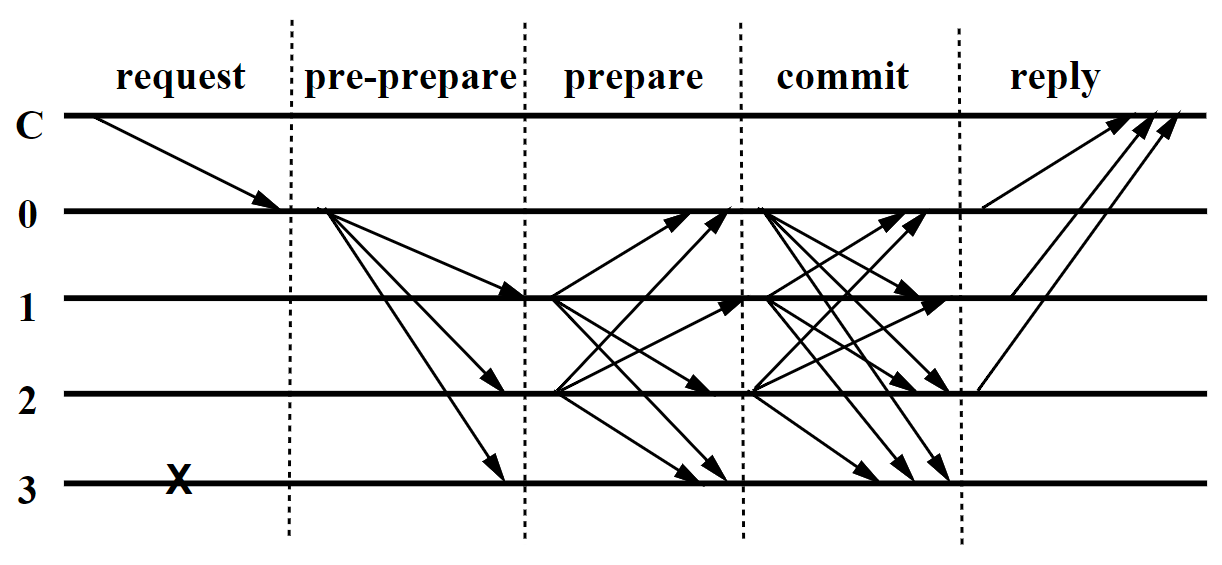
\includegraphics[width=1\textwidth]{pbft.eps}
\caption{정상 케이스 동작(Normal Case Operation)}
\label{fig:1}       %Give a unique label
\end{figure}

\subsection{HotStuff: BFT Consensus with Linearity and Responsiveness}

\subsection{LibraBFT: BFT Consensus with Linearity and Responsiveness}
LibraBFT는 Libra 블록체인을 위해 비동기 네트워크 환경에서 safety속성을 보장하는 비잔틴 장애 허용 합의 알고리즘이다.
지리적으로 분산된 데이터베이스 간에 상태 머신 복제를 통해 동일한 프로그래밍 가능한 리소스(programmable resources)을
유지할 수 있게한다. 다른 상태 머신 복제 알고리즘과 유사하게 
각 데이터베이스는 순서있는 트랜잭션 목록을 받고 실행하여 동일한 상태를 유지한다.
 이 합의 알고리즘 역시 다른 알고리즘 처럼 \(3f+1\) 개의 노드가 있어야 시스템을 비잔틴 행위로 부터
시스템을 보호할 수 있다. LibraBFT는 HotStuff 알고리즘을 기반으로하는 알고리즘이다. HotStuff 장점으로 다음이 있다.
\begin{itemize}
  \item 합의 결정 비용은 단순히 결정을 각 복제본에 전파하는 것 이상의 비용이 들지 않는다.
  \item 단일 통신 단계를 중심으로 프로토콜이 구축되어 간결하면서도 견고한 블록체인 구현을 할 수 있게 한다.
  \item 공개 모집을 통해 새롭게 모집된 노드를 동적으로 시스템에 추가할 수 있다. 
\end{itemize}

LibraBFT는 전통적인 라운드 방식을 적용하며 특히 HotStuff의 3단계 합의 방식을 사용한다. 기본적으로 
각 라운드는 여러개의 단계로 구성되며 이는 라운드 단위로 리더를 지정하고 
리더가 제안하게 하고 결함없는 검증자가 라운드의 여러 단계에 참여하는 방식이다. 
첫번째와 두번째 단계에서는 쿼럼 인증서를 만들고 2개의 쿼럼 인증서 체인에 대한 합의가 이뤄지면 커밋에 도달하는 식이다.
이 방식을 통해 LibraBFT는 낙관적 응답성(optimistic reponsiveness)와 선형성(linearity)을 보장할 수 있다. 

LibraBFT는 체이닝(Chaining) 패러다임을 차용하고 있다. LibraBFT의 3단계는 각 라운드에 퍼져있다.
예를들어 k라운드에서 리더는 제안에 대한 인증을 진행한다.
여기서 인증은 쿼럼인증서 생성을 의미한다. k+1 라운드에서는 리더는 제안에 대한 인증을 진행한다.
동시에 k라운드 쿼럼 인증서에 대한 인증을 진행한다. 따라서 k+1 라운드는 k+1에 대한 쿼럼인증서와 
k라운드 제안의 쿼럼인증서의 쿼럼인증서를 생성한다. k+2 라운드에서는 쿼럼인증서 생성 뿐만 아니라 k라운드 제안은
커밋될 수 있는 상태가 된다. Figure ~\ref{fig:2} 와 같이 k+3 라운드가 시작되면서 k라운드에 제안된 명령은
HotStuff의 DECIDE 단계에 도달하게 되어 명령이 실행되고 커밋된다.

LibraBFT는 리더 기반 알고리즘으로 커밋까지 \(O(n)\) 정도의 메시지 통신 비용이 발생한다. 그리고 비잔틴 노드나
장애로 인해 특정 라운드가 타웃아웃 되더라도 동일하게 \(O(n)\) 의 메시지 통신 비용이 발생한다.



\begin{figure}
  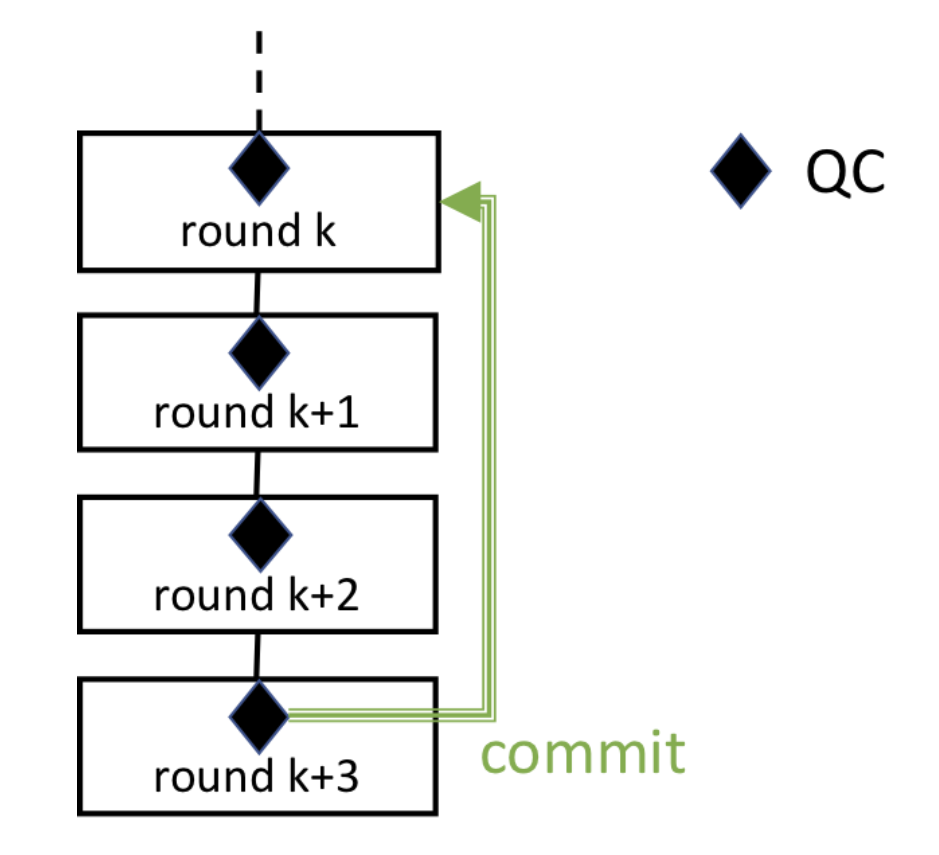
\includegraphics[width=0.5\textwidth]{librabft.eps}
\caption{LibraBFT 단계들은 여러 라운드에 펼쳐져 있음}
\label{fig:2}       %Give a unique label
\end{figure}


%Text with citations \cite{RefB} and \cite{RefJ}.
\subsection{Subsection title}
\label{sec:11}
as required. Don't forget to give each section
and subsection a unique label (see Sect.~\ref{sec:1}).
\paragraph{Paragraph headings} Use paragraph headings as needed.qwd 
\begin{equation}
a^2+b^2=c^2
\end{equation}

% For one-column wide figures use
  %\begin{figure}
% Use the relevant command to insert your figure file.
% For example, with the graphicx package use
     %
\includegraphics{example.eps}
% figure caption is below the figure
  %\caption{Please write your figure caption here}
  %\label{fig:1}       % Give a unique label
  %\end{figure}
%
% For two-column wide figures use
%
% For tables use
  %\begin{table}
% table caption is above the table
  %\caption{Please write your table caption here}
  %\label{tab:1}       % Give a unique label
% For LaTeX tables use
  %\begin{tabular}{lll}
  %\hline\noalign{\smallskip}
  %first & second & third  \\
  %\noalign{\smallskip}\hline\noalign{\smallskip}
  %number & number & number \\
  %number & number & number \\
  %\noalign{\smallskip}\hline
  %\end{tabular}
  %\end{table}

\section{토론}
\label{sec:2}
%Text with citations \cite{RefB} and \cite{RefJ}.
asd asdasd
\section{결론}
\label{sec:3}
%Text with citations \cite{RefB} and \cite{RefJ}.

%\begin{acknowledgements}
%If you'd like to thank anyone, place your comments here
%and remove the percent signs.
%\end{acknowledgements}


% Authors must disclose all relationships or interests that 
% could have direct or potential influence or impart bias on 
% the work: 
%
% \section*{Conflict of interest}
%
% The authors declare th at they have no conflict of interest.


% BibTeX users please use one of
%\bibliographystyle{spbasic}      % basic style, author-year citations
%\bibliographystyle{spmpsci}      % mathematics and physical sciences
\bibliographystyle{spphys}       % APS-like style for physics
\bibliography{test}         % qhe.bib is the name of our database
% name your BibTeX data base asd

% Non-BibTeX users please use  
  %\begin{thebibliography}{asdf}
%
% and use \bibitem to create references. Consult the Instructions
% for authors for reference list style.
%
  %\bibitem{RefJ}
% Format for Journal Reference
  %Author, Article title, Journal, Volume, page numbers (year)
% Format for books
  %\bibitem{RefB}
  %Author, Book title, page numbers. Publisher, place (year)
% etc
  %\end{thebibliography}
        % qhe.bib is the name of our database
     
\end{document}
% end of file template.tex

